% $Id: INF_Poster_example.tex 7714 2011-08-31 17:34:46Z tkren $
%
% TU Wien - Faculty of Informatics
% poster template
%
% This template is using the beamer document class and beamerposter package, see
% <http://www.ctan.org/tex-archive/macros/latex/contrib/beamer/>
% <http://www.ctan.org/tex-archive/macros/latex/contrib/beamerposter/>
% <http://www-i6.informatik.rwth-aachen.de/~dreuw/latexbeamerposter.php>
%
% For questions and comments send an email to
% Thomas Krennwallner <tkren@kr.tuwien.ac.at>
%

\documentclass[final,hyperref={pdfpagelabels=true}]{beamer}

\usepackage{TUINFPST}
\usepackage{listings}

%\title[Computational Intelligence]{Interactive Computer Generated Architecture}
% if you have a long title looking squeezed on the poster, just force
% some distance:
\title[Software Engineering \& Internet Computing]{%
  A Weather Ontology for \\[0.2\baselineskip]%
  Predictive Control in Smart Homes %\\[0.2\baselineskip]%
}
\author[paulchen@rueckgr.at]{Paul Staroch}
\institute[]{%
  Technische Universit{\"a}t Wien\\[0.25\baselineskip]
  Institut für computergestützte Automation\\[0.25\baselineskip]
  Arbeitsbereich: Automation Systems Group\\[0.25\baselineskip]
  BetreuerIn: Ao.Univ.-Prof. Dipl.-Ing. Dr.techn. Wolfgang Kastner\\[0.25\baselineskip]
  AssistentIn: Dipl.-Ing. Mario Kofler
}
\titlegraphic{
\includegraphics[height=52mm]{figures/183-1.pdf}}
\date[\today]{\today}
\subject{epilog}
\keywords{my kwd1, my kwd2} % TODO

%%%%%%%%%%%%%%%%%%%%%%%%%%%%%%%%%%%%%%%%%%%%%%%%%%%%%%%%%%%%%%%%%%%%%%%%%%%%%%%%%%%%%%

% Display a grid to help align images 
\beamertemplategridbackground[12.7mm] % TODO remove

% play around with the background colors
% \setbeamercolor{background canvas}{bg=yellow}

% use a background picture
%\usebackgroundtemplate{%
%  
\includegraphics[width=\paperwidth]{logo_KBS_2_CMYK}
%}

% play around with block colors
\setbeamercolor{block body}{fg=black,bg=white}
\setbeamercolor{block title}{fg=TuWienBlue,bg=white}

\definecolor{TuWienBlueLight}{cmyk}{.1,.1,.1,.3}

\setbeamertemplate{block begin}{
  \begin{beamercolorbox}{block title}%
    \begin{tikzpicture}%
      \node[draw,rectangle,line width=3pt,rounded corners=0pt,inner sep=0pt,shade,top color=white,bottom color=TuWienBlueLight]{%
        \begin{minipage}[c][2cm]{\linewidth}
          \centering\textbf{\insertblocktitle}
        \end{minipage}
      };
    \end{tikzpicture}%
  \end{beamercolorbox}
  \vspace*{1cm}
  \begin{beamercolorbox}{block body}%
}

\setbeamertemplate{block end}{
  \end{beamercolorbox}
  \vspace{2cm}
}

% setup postit
\setbeamercolor{postit}{fg=black,bg=yellow} 
\newenvironment{postit}
{\begin{beamercolorbox}[sep=1em,wd=7cm]{postit}}
{\end{beamercolorbox}}


% for crop marks, uncomment the following line
\usepackage[cross,width=88truecm,height=123truecm,center]{crop}

%%%%%%%%%%%%%%%%%%%%%%%%%%%%%%%%%%%%%%%%%%%%%%%%%%%%%%%%%%%%%%%%%%%%%%%%%%%%%%%%%%%%%%

%\lstset{frame=trbl,basicstyle=\scriptsize,moredelim=**[is][{\btHL[fill=green!20]}]{@@}{@@},}
\lstset{frame=trBL,basicstyle=\normalsize}

% \setlength{\parskip}{15em}

\begin{document}

% We have a single poster frame.
\begin{frame}[fragile]
  \begin{columns}[t]
    % ---------------------------------------------------------%
    % Set up a column
    \begin{column}{.45\textwidth}
      \begin{block}{Why introduce smart homes?}
	\emph{Smart homes} are dwellings that are equipped with
	some kind of intelligence that enables them to perform tasks
	on its own without human intervention. Some of their goals are:

	\begin{itemize}
	  \item Supporting the inhabitants in their routine tasks.
	  \item Maintaining or increase the inhabitant's comfort.
          \item Reducing the overall energy consumption.
        \end{itemize}

	Areas served by smart homes include … % TODO

%	Components of smart homes are \emph{sensors} which provide
%	data about the current state, while \emph{actuators} can
%	execute various tasks. \emph{Intelligent control} represents
%	a gateway for managing the systems via an \emph{internal
%	network}. % TODO replace this by an image or omit it completely?
      \end{block}

      \begin{block}{Why use ontologies?}
	Many smart home systems suffer from several shortcomings, e.g.
	\begin{itemize}
	  \item … % TODO
	  \item … % TODO
	  \item … % TODO
	\end{itemize}

	Smart home environments such as \emph{ThinkHome}~\cite{CR2011-TH_Journal}
	aim to overcome these problems by utilising a knowledge base
	built using \emph{OWL}.
        % TODO 
	% logical model, OWL, ThinkHome
      \end{block}

      \begin{block}{Why add a weather data model?}
	Without question, weather has a wide influence on a dwelling.
	Introducing a data model for current and future weather states
	enables a smart home to utilise various aspects of this
	influence to make a set of control decisions, e.g.:
	\begin{itemize}
	  \item foo
	  \item bar
	  \item blah
	  \item blubb
	  \item Prepare for severe weather, e.g. by closing windows or retracting awnings.
	\end{itemize}

	Data about weather states is gathered from local sensors and Internet weather services.
      \end{block}

      \begin{block}{Preliminary work}
	Evaluation of existing work yielded to the following insights: % TODO
	\begin{itemize}
	  \item \emph{METHONTOLOGY} is selected as approach creating a weather data ontology.
	  \item The weather elements supported by the ontology are temperature, humidity, … % TODO
	  \item The \emph{API} of the \emph{Norwegian Meteorological Institute} is used as an example for an Internet weather service.
	\end{itemize}
      \end{block}

      \begin{block}{The \emph{SmartHomeWeather} ontology}
	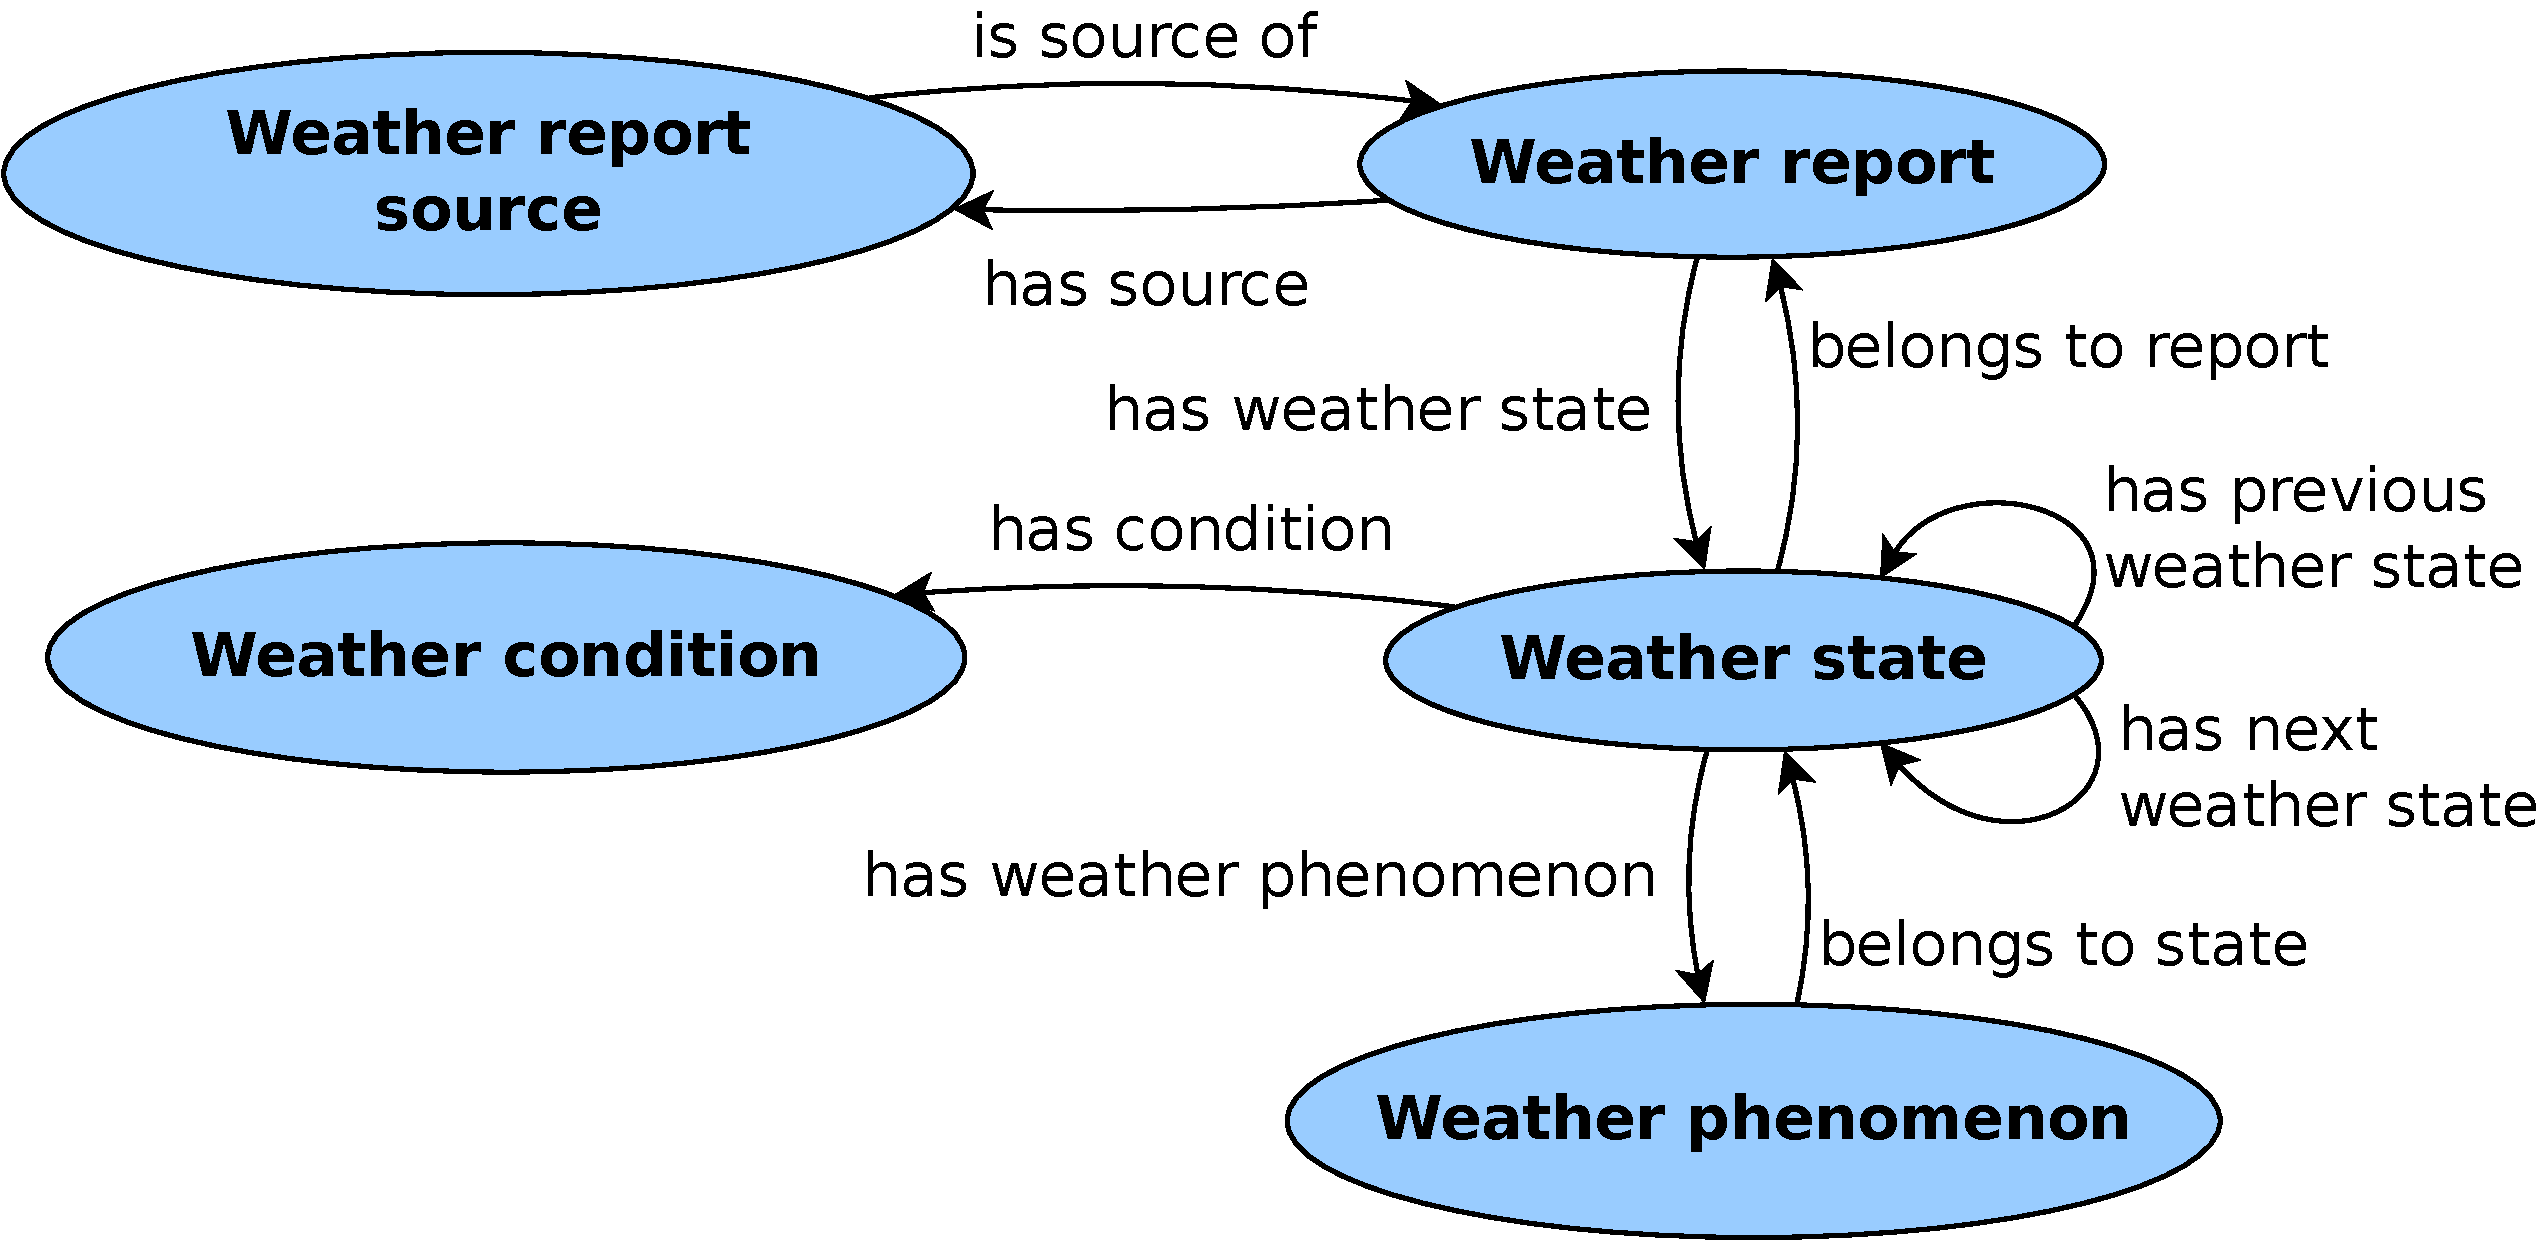
\includegraphics[width=\textwidth]{figures/binary-relations.pdf}
      \end{block}
    \end{column}
    % ---------------------------------------------------------%
    % end the column

    % ---------------------------------------------------------%
    % Set up a column 
    \begin{column}{.45\textwidth}
      \begin{block}{The \emph{SmartHomeWeather} ontology (cont.)}
	The \emph{SmartHomeWeather} ontology is built around five top-level concepts which together with their sub-concepts form a model for maintaining data about current and future weather and perform efficient \emph{OWL} reasoning on it:
	\begin{itemize}
          \item ...
          \item ...
          \item ...
          \item ...
          \item ...
	\end{itemize}

	Sub-concepts of \emph{Weather phenomenon} are defined using \emph{OWL} axioms:

	\begin{lstlisting}
RoomTemperature :- WeatherPhenomenon and
        hasTemperature >= 20 and
        hasTemperature <= 25
	\end{lstlisting}

	Sub-concepts of \emph{Weather state} are defined in a similar way:

	\begin{lstlisting}
	WindyWeather :- something
	\end{lstlisting}

	Due to limitations of \emph{OWL} (\emph{Open-World Assumption}), some ... are retrieved using \emph{SPARQL} queries: % TODO though not part of \emph{SmartHomeWeather}

	\begin{lstlisting}
	blah
	\end{lstlisting}

	\emph{SWRL} rules are used as well:

	\begin{lstlisting}
	blah
        \end{lstlisting}
      \end{block}

      \begin{block}{The Weather Importer}
	% TODO
      \end{block}

      \begin{block}{Future work}
	Interoperation with other data sources:
	\begin{itemize}
	  \item … % TODO
	  \item … % TODO
	  \item … % TODO
	\end{itemize}
      \end{block}

      \begin{block}{References}
	\bibliographystyle{thesis}
	\bibliography{references}

	% TODO owl, thinkhome, ontologies, ...?
      \end{block}
    \end{column}
    % ---------------------------------------------------------%
    % end the column
  \end{columns}

%  \begin{tikzpicture}[remember picture,overlay]
%    \node[inner sep=0pt,xshift=-30cm,yshift=23cm] at (current page.east) {%
%      \begin{postit}%
%        Post-It time!%
%      \end{postit}%
%    }; 
%  \end{tikzpicture}
  
\end{frame}

\end{document}

%%% Local Variables:
%%% TeX-PDF-mode: t
%%% TeX-debug-bad-boxes: t
%%% TeX-master: t
%%% TeX-parse-self: t
%%% TeX-auto-save: t
%%% reftex-plug-into-AUCTeX: t
%%% End:
